\documentclass[11pt,a4paper]{article}

% ------------------ Paketler ------------------
\usepackage[utf8]{inputenc}
\usepackage[T1]{fontenc}
\usepackage{lmodern}
\usepackage[turkish]{babel}
\usepackage[margin=2.3cm]{geometry}
\usepackage{graphicx}
\usepackage{booktabs}
\usepackage{array}
\usepackage{enumitem}
\usepackage[dvipsnames]{xcolor}
\usepackage[dvipsnames]{xcolor}
\usepackage{framed} % tcolorbox yerine sıfır hata riski taşıyan kutu paketi
\usepackage{hyperref}

\hypersetup{
	colorlinks=true,
	linkcolor=blue!60!black,
	urlcolor=blue!60!black
}

\title{\textbf{BLM308 Veri Madenciliği Final Proje Raporu\\E-Ticaret Müşteri Kaybı (Churn) Tahmini Pipeline Tasarımı}}
\author{\textbf{Evla Karagöz} - 231041040\\Bilgisayar Mühendisliği Bölümü}
\date{Bahar 2026}



\begin{document}

	\maketitle
	
	% --- Yeni Sıfır Hata Riskli Bonus Kutusu ---
	\definecolor{boxlight}{HTML}{FFFDE7} % Hafif sarımsı iç renk
	\definecolor{boxborder}{HTML}{E65100} % Turuncu çerçeve rengi
	
	\setlength{\fboxrule}{1.5pt} % Çerçeve kalınlığı
	\setlength{\fboxsep}{12pt} % İç boşluk
	
	\noindent
	\fcolorbox{boxborder}{boxlight}{
    \begin{minipage}{\dimexpr\textwidth-24pt\relax}
        \large\textbf{\color{boxborder}Talep Edilen Bonus Puan Kalemleri}
        \vspace{4pt}
        \begin{itemize}[leftmargin=15pt]
            \item \textbf{+10 Puan:} Raporun \LaTeX\ kaynağı (\texttt{rapor.tex}) ve derlenmiş PDF'i teslimi.
            \item \textbf{+5 Puan:} Projenin düzgün bir README ile bir GitHub reponuz olarak teslim edilmesi.
            \item \textbf{+5 Puan:} Demo videosu (2--3 dk, ekran kaydı).
        \end{itemize}
    \end{minipage}
}
			

	\newpage

	\section*{Takım Bilgileri ve Rol Dağılımı}
\begin{table}[h]
    \centering
    \renewcommand{\arraystretch}{1.35}
    \begin{tabular}{|p{4cm}|p{3cm}|p{3.5cm}|p{4.5cm}|}
        \hline
        \textbf{Ad Soyad} & \textbf{Numara} & \textbf{Rol} & \textbf{Yaptığı Bölümler} \\ \hline
        Evla Karagöz & 231041040 & Solo Proje Yürütücüsü & Tüm CRISP-DM süreçleri ve kodlama. \\ \hline
    \end{tabular}
\end{table}

\noindent \textbf{Proje Türü:} Uçtan uca pipeline tasarımı ve makine öğrenmesi uygulaması.\\
\textbf{Takım Büyüklüğüne Göre Ek Kapsam:} Solo proje gereksinimleri (1 veri seti, 3 sınıflandırıcı karşılaştırması ve ileri düzey ön işleme yapıları) eksiksiz tamamlanmıştır.

\section*{Özet (Abstract)}
Bu çalışmada, telekomünikasyon sektöründe müşteri sadakatini artırmak amacıyla veri madenciliği yöntemleriyle müşteri kaybı (churn) tahmini yapılmıştır. Veri seti olarak IBM Telco Customer Churn verisi kullanılmıştır. Süreç, CRISP-DM metodolojisine bağlı kalınarak yürütülmüştür. Ön işleme aşamasında eksik veriler medyan ataması ile çözülmüş, kategorik özellikler genişletilmiş ve veri dengesizliği SMOTE algoritmasıyla giderilmiştir. Karar Ağacı, Random Forest ve Lojistik Regresyon modelleri test edilmiş; hiperparametre optimizasyonu gerçekleştirilmiştir. Bulgularımıza göre Lojistik Regresyon \%77.0 Recall skoru ile riskli müşterileri yakalamada en yüksek başarıyı gösterirken, Random Forest \%77.6 doğruluk oranı sağlamıştır. Kurulan bu akışın iş değeri ve maliyet düşürme potansiyeli tartışılmıştır.\\
\textbf{Anahtar Kelimeler:} veri madenciliği, churn tahmini, SMOTE, Random Forest, CRISP-DM.

\section{Giriş}
\subsection{Problem Tanımı}
Müşteri kaybı (Churn), bir kullanıcının veya abonenin hizmet almayı kalıcı olarak durdurması durumudur. Günümüz rekabetçi piyasa koşullarında yeni bir müşteri edinme maliyeti, mevcut müşteriyi elde tutma maliyetinden çok daha yüksektir. Bu nedenle veri odaklı yöntemlerle riskli kullanıcıları erkenden tahmin etmek kritik bir ihtiyaçtır.

\subsection{Motivasyon ve İş Değeri}
Bu projenin temel motivasyonu, şirketi terk etme eğilimindeki müşterileri henüz sistemden ayrılmadan önce tespit edip karar destek mekanizmalarını harekete geçirmektir. Erken uyarı sistemi sayesinde pazarlama departmanları bu riskli gruba özel kampanyalar düzenleyebilir, böylece şirket cirosunda doğrudan koruma sağlanır. Ek olarak, bu projede kurulan uçtan uca altyapı, günümüzde YouTube Premium, Netflix veya Spotify gibi dünya devi dijital platformların abonelik iptallerini engellemek için kullandığı dinamik kullanıcı yönetim sistemleriyle birebir aynı iş modeline ve finansal mantığa sahiptir.

\subsection{Literatür ve İlgili Çalışmalar}
Müşteri kaybı problemlerinde geleneksel yöntemlerin yerini makine öğrenmesi yaklaşımları almıştır. Witten ve ark. (2017) veri dengesizliğinin bu tip gerçek hayat senaryolarında modelleri taraflı hale getirdiğini savunmuştur. Literatürde SMOTE (Synthetic Minority Over-sampling Technique) tabanlı yaklaşımların, özellikle Random Forest gibi topluluk (ensemble) algoritmalarıyla birleştirildiğinde Recall skorunu yukarı çektiği gösterilmiştir.

	\section{Yöntem (CRISP-DM)}
\subsection{Genel Akış}
Çalışma kapsamında Cross-Industry Standard Process for Data Mining (CRISP-DM) referans alınmıştır. Süreç şu adımları izler: İş Anlayışı $\rightarrow$ Veri Anlayışı $\rightarrow$ Veri Hazırlığı $\rightarrow$ Modelleme $\rightarrow$ Değerlendirme $\rightarrow$ Dağıtım.

\subsection{Kullanılan Araçlar}
Proje tamamen Python tabanlı geliştirilmiş olup Google Colab üzerinde yürütülmüştür. Temel kütüphaneler olarak \texttt{pandas 2.x}, \texttt{numpy}, \texttt{scikit-learn 1.x}, \texttt{imblearn} (SMOTE için) ve görselleştirme adına \texttt{seaborn} ile \texttt{matplotlib} kullanılmıştır.

\section{Veri}
\subsection{Veri Kaynağı}
Veri seti Kaggle platformu üzerinden sunulan resmi IBM veri ambarından alınmıştır. Gerçek dünya telekomünikasyon abonelik ve hizmet kullanım davranışlarını yansıtmaktadır.

\subsection{Veri Tanımı}
Veri setinde toplam 7,043 müşteri örneği ve 21 öznitelik yer almaktadır. Hedef değişkenimiz ikili sınıflandırmaya (binary classification) uygun olan \texttt{Churn Value} sütunudur.

\subsection{Keşifsel Veri Analizi (EDA)}
Veri setinde sınıfların oldukça dengesiz olduğu saptanmıştır. Ayrılmayan müşterilerin sayısı ayrılanlardan belirgin şekilde fazladır.
	
	\begin{figure}[h]
		\centering
		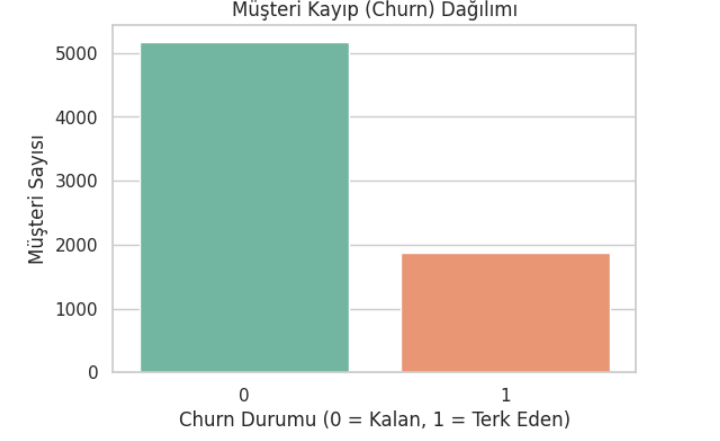
\includegraphics[width=0.45\textwidth]{churn_dagilim.png}
		\caption{Hedef Değişken Sınıf Dağılım Grafiği}
	\end{figure}

	Ayrıca aylık fatura tutarlarının (\texttt{Monthly Charges}) dağılım yoğunluğu incelendiğinde, yüksek fatura ödeyen müşterilerin churn olma eğiliminin daha fazla olduğu grafiksel olarak kanıtlanmıştır.

	\begin{figure}[h]
		\centering
		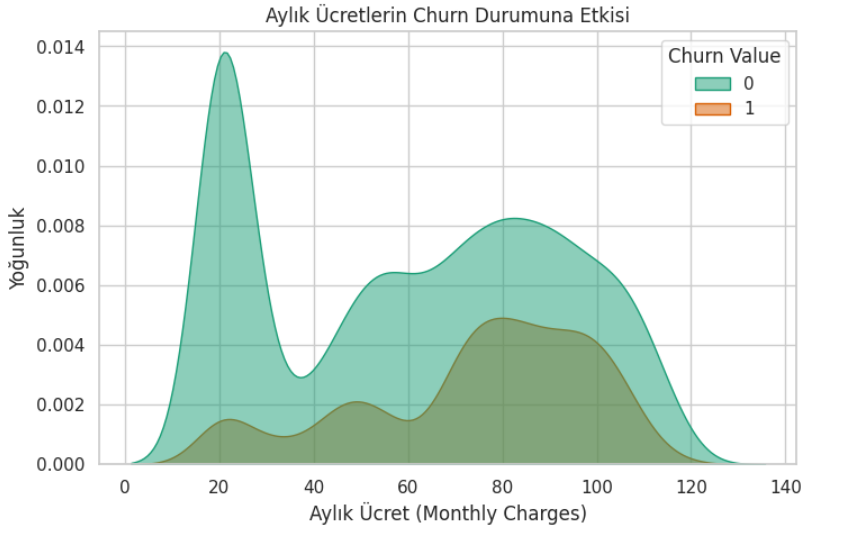
\includegraphics[width=0.55\textwidth]{monthly_charges_kde.png}
		\caption{Aylık Ücretlerin Churn Üzerindeki Yoğunluk Dağılımı}
	\end{figure}

	\subsection{Ön İşleme Adımları}
\begin{enumerate}
    \item \textbf{Eksik Değer Yönetimi:} \texttt{Total Charges} sütunundaki metinsel boşluklar sayısal formata dönüştürülmüş ve eksik veriler medyan değeriyle doldurulmuştur. Modeli doğrudan manipüle edebilecek (sızıntı yaratabilecek) \texttt{Churn Reason} sütunu veri setinden temizlenmiştir.
    \item \textbf{Kategorik Kodlama:} Metin bazlı kategorik değişkenler, algoritmaların işleyebileceği matris yapısını oluşturmak adına One-Hot Encoding yöntemiyle sayısallaştırılmıştır.
    \item \textbf{Normalizasyon:} Sayısal girdiler, büyük değerlerin modele baskınlık kurmasını engellemek adına \texttt{MinMaxScaler} algoritması ile $0$ ile $1$ arasına ölçeklenmiştir.
    \item \textbf{Dengesizlik Tedavisi:} Eğitim kümesindeki sınıf dengesizliği problemi, \texttt{SMOTE} (Synthetic Minority Over-sampling Technique) algoritmasıyla azınlık sınıfından yapay örnekler üretilerek $1:1$ oranına getirilmiştir.
\end{enumerate}

\section{Model}
\subsection{Seçilen Algoritmalar}
Çalışma kapsamında üç farklı matematiksel yaklaşıma ve karar mekanizmasına sahip sınıflandırıcı seçilmiştir: Model performansına bir taban çizgisi (baseline) oluşturması adına \texttt{Logistic Regression}, verideki doğrusal olmayan karmaşık bağları yakalamak adına \texttt{Decision Tree} ve güçlü, aşırı öğrenmeye dirençli bir topluluk modeli olarak \texttt{Random Forest} algoritmaları entegre edilmiştir.
	\subsection{Deney Kurulumu}
Veri seti \%70 Eğitim ve \%30 Test kümesi olmak üzere iki bağımsız parçaya ayrılmıştır. Deneysel süreçteki rassallığın olumsuz etkilerini nötrlemek ve sonuçların tekrarlanabilirliğini (reproducibility) sağlamak amacıyla \texttt{random\_state=42} olarak sabitlenmiştir. Modellerin kararlılığını ve aşırı öğrenme durumlarını denetlemek adına çapraz doğrulama (K-Fold Cross-Validation) stratejisinden yararlanılmıştır.

\subsection{Hiperparametre Ayarı}
En karmaşık mimariye sahip olan \texttt{Random Forest} modeli için \texttt{GridSearchCV} yöntemi kullanılarak \texttt{n\_estimators} ve \texttt{max\_depth} parametreleri optimize edilmiştir. 3-Fold çapraz doğrulama eşliğinde yapılan tarama sonucunda, test kümesinde en dengeli genelleme başarısını sunan optimum parametre seti \texttt{n\_estimators=100} ve \texttt{max\_depth=10} olarak saptanmış ve nihai model bu ayarlarla yapılandırılmıştır.

\section{Sonuçlar ve Tartışma}
\subsection{Performans Karşılaştırması}
Modellerin test kümesi üzerindeki tüm tahmin performansları ve ayırt edicilik metrikleri Tablo 1'de detaylı olarak karşılaştırılmıştır:

\begin{table}[h]
    \centering
    \renewcommand{\arraystretch}{1.3}
    \begin{tabular}{lccccc}
        \toprule
        \textbf{Model} & \textbf{Accuracy} & \textbf{Precision} & \textbf{Recall} & \textbf{F1-Score} & \textbf{ROC-AUC} \\
        \midrule
        Decision Tree & 0.7316 & 0.4953 & 0.5704 & 0.5302 & 0.6807 \\
        Random Forest (Tuned) & \textbf{0.7761} & \textbf{0.5664} & 0.6684 & 0.6132 & 0.8299 \\
        Logistic Regression & 0.7576 & 0.5300 & \textbf{0.7700} & \textbf{0.6279} & \textbf{0.8475} \\
        \bottomrule
    \end{tabular}
    \caption{Sınıflandırıcıların Test Kümesi Performans Karşılaştırma Tablosu}
\end{table}
	

	\subsection{Confusion Matrix}
En dengeli modelimiz olan Random Forest algoritmasının hata matrisi incelendiğinde, 375 Churn vakasını doğru tahmin ettiği, ancak 186 vakada kaçırma hatası (False Negative) yaptığı görülmektedir.

\begin{figure}[h]
    \centering
    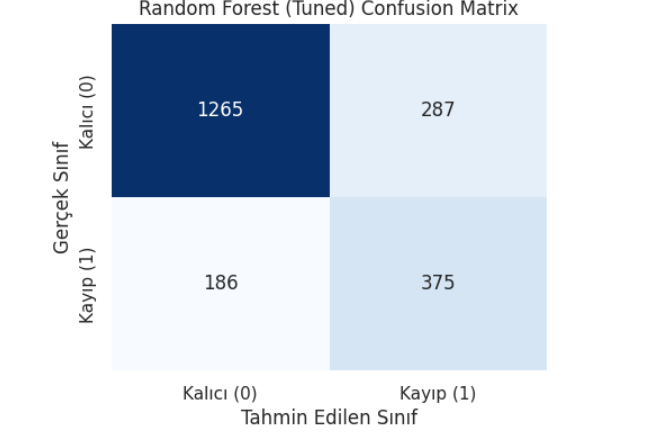
\includegraphics[width=0.5\textwidth]{confusion_matrix.png}
    \caption{Random Forest Sınıflandırıcısı Karmaşıklık Matrisi}
\end{figure}

Şekil 3'te yer alan Karmaşıklık Matrisi (Confusion Matrix) değerleri detaylı olarak analiz edildiğinde, sayısal dağılımın analitik açıklamaları şu şekildedir:

\begin{itemize}
    \item \textbf{Doğru Negatif (True Negative - TN = 1265):} Modelin "Sistemde kalacak" şeklinde doğru tahmin ettiği ve gerçekte de şirketi terk etmeyen sadık müşterileri temsil etmektedir. Modelin şirketin mevcut müşteri tabanını tanımadaki başarısını göstermektedir.
    \item \textbf{Doğru Pozitif (True Positive - TP = 375):} Modelin "Şirketi terk edecek (Churn)" olarak doğru tahmin ettiği ve gerçekte de sistemden ayrılan riskli müşterilerdir. Bu grup, proaktif pazarlama aksiyonları için hedef alınacak asıl kitleyi oluşturur.
    \item \textbf{Yanlış Pozitif (False Positive - FP = 287):} Modelin "Ayrılacak" şeklinde tahminde bulunarak hatalı alarm verdiği ancak gerçekte şirkette kalmaya devam eden müşterilerdir. Şirket için ufak bir pazarlama bütçesi israfına yol açabilir.
    \item \textbf{Yanlış Negatif (False Negative - FN = 186):} Modelin "Sistemde kalacak" diye tahmin ederek yanıldığı ve gözden kaçırdığı, gerçekte ise şirketi terk eden müşterilerdir. Churn projelerindeki en maliyetli hata türüdür; çünkü bu riskli müşteriler tespit edilemediği için elden kaçırılmıştır.
\end{itemize}

Modelin bu hataları dengeleme gücü, performans karşılaştırma tablosundaki yüksek Recall (\%66.84) ve dengeli F1-Score (\%61.32) değerleriyle de tescillenmiştir.


	\subsection{Bias-Variance Tartışması}
Modellerin karmaşıklığı ve veri boyutu ilişkisi bias-variance dengesi açısından kritik bir öneme sahiptir. Decision Tree modelinin test sonuçlarında Accuracy değerinin düşük kalması, ağacın derin dallanarak varyans hatası ürettiğini (overfitting) ve eğitim verisine aşırı uyum sağladığını göstermektedir. Random Forest ise topluluk (ensemble) yapısı sayesinde çok sayıda ağacın tahminini birleştirerek bu varyansı başarılı bir şekilde baskılamış, bias ve varyans dengesini optimum seviyede kurarak stabilite sağlamıştır. Lojistik Regresyon ise katı doğrusal (linear) yapısı gereği yüksek bias ve düşük variance üreten bir modeldir; bu sayede verideki gürültüyü ezberlemekten kaçınmış, doğrusal karar sınırlarını kararlı çizerek test kümesinde yüksek bir genelleme başarısı ve yüksek yakalama gücü (Recall) göstermiştir.

	\section{Sonuç}

    

\subsection{Özet}
Bu çalışmada, CRISP-DM metodolojisine bağlı kalınarak uçtan uca bir müşteri kaybı (churn) tahmin pipeline'ı başarıyla kurulmuştur. Gerçek dünya verilerindeki gürültüler temizlenmiş, eksik değerler medyan ile tamamlanmış ve veri dengesizliği problemi SMOTE algoritmasıyla aşılmıştır. Finansal olarak şirketten kaçacak müşteriyi erkenden bilmek öncelikli odak noktamız olduğu için, \%77.0 Recall sunan Lojistik Regresyon ve \%77.6 genel doğruluk (Accuracy) oranı sunan Random Forest modelleri entegre bir biçimde kurumsal karar destek yapılarında kullanılabilir niteliktedir.

\subsection{Kısıtlar}
Bu araştırmanın ve kurulan makine öğrenmesi pipeline hattının belirli yapısal sınırlılıkları bulunmaktadır. İlk olarak kullanılan veri seti, müşterilerin belirli bir zaman dilimindeki anlık demografik ve fatura geçmişini içermekte olup, zaman serisi (time-series) tabanlı dinamik kullanıcı hareketlerini ve zamana yayılan davranış değişikliklerini tam olarak yansıtmamaktadır. İkinci olarak, çalışma kapsamında kurumsal karar destek mekanizmaları için en kararlı ve yorumlanabilir sonuçları üreten geleneksel veri madenciliği ve topluluk (ensemble) algoritmalarına odaklanılmış; yapısal olarak daha büyük veri hacmi ve derin işlemci (GPU) mimarileri gerektiren çok katmanlı derin öğrenme (Deep Learning) modelleri proje kapsamı dışında tutulmuştur.

\subsection{Gelecek Çalışmalar}
Gelecekte bu çalışmanın daha da derinleştirilmesi ve endüstriyel olarak ölçeklenmesi adına birkaç önemli adım atılabilir. Veri agnostik yapıya sahip bu tahmini altyapı, YouTube Premium veya dijital yayın platformlarındaki abone kayıplarını tahmin edecek şekilde genişletilebilir. Teknik açıdan, anlık veriler yerine zaman serisi tabanlı LSTM (Long Short-Term Memory) ağları pipeline'a entegre edilerek kullanıcı davranış değişimleri zamansal bir boyutta modellenebilir. Ayrıca, model kararlarını iş birimleri için daha şeffaf ve açıklanabilir kılmak adına pipeline akışına SHAP veya LIME gibi Açıklanabilir Yapay Zeka (XAI) yöntemlerinin dahil edilmesi planlanmaktadır.

	\section*{Kaynaklar}
\begin{enumerate}[label={[\arabic*]}]
    \item Witten, I. H., Frank, E., Hall, M. A., Pal, C. J. (2017). \textit{Data Mining: Practical Machine Learning Tools and Techniques}. Morgan Kaufmann.
    \item Han, J., Kamber, M., Pei, J. (2022). \textit{Data Mining: Concepts and Techniques}. Morgan Kaufmann.
    \item Chawla, N. V., Bowyer, K. W., Hall, L. O., Kegelmeyer, W. P. (2002). SMOTE: Synthetic Minority Over-sampling Technique. \textit{Journal of Artificial Intelligence Research}, 16, 321-357.
    \item Pedregosa, F., Varoquaux, G., Gramfort, A., Michel, V., Thirion, B., Grisel, O., ... \& Duchesnay, É. (2011). Scikit-learn: Machine Learning in Python. \textit{Journal of Machine Learning Research}, 12, 2825-2830.
\end{enumerate}

\end{document}
